\chapter{A New Perspective}

\begin{summary}
  Here, we will loosely introduce the notion of a fractal, where interest in fractals stems from, and some various ways one can think about the geometries of their defining sets. 
\end{summary}

\section{Introduction to Fractals}
Homo sapiens, as early as the Neanderthals, were able to recognize that paths covering a longer distance would take more time to travel. Or more generally, not all paths that connect point $A$ to point $B$ are equal in length. However, even at this time, there did not exist any way to actually measure distances, let alone a numerical system to compare distances that differed. Contemporary humans have developed an innumerate number of methods to calculate the length of a given path. \\

\begin{wrapfigure}{r}{0.6\textwidth}
  \begin{center}
    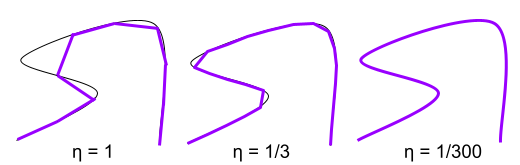
\includegraphics[width=0.6\textwidth]{Images/1.1.png}
  \end{center}
  \caption{Approximating length of a curve}
\end{wrapfigure}

How would you choose to calculate the length of the curve to the right? When it comes to nonlinear paths, finding the length is not exactly as intuitive of holding a ruler against it, although one could lay out a string over the curve, pick up the string holding it straight, and measure the resulting line. A more mathematically analytical take would be to place ``rulers'' of length $\eta$ along the curve using as few as possible. By multiplying the number of rulers by the length of each $(\eta)$, we can generate an approximation for the length of the curve, which we denote $\lambda$. \\


As $(\eta)$ becomes smaller and smaller, the number of rulers becomes increasingly large. Although, we expect that the product $\lambda$ would converge to a particular real value, the true length of the curve. Curves such that $\displaystyle \lim_{\eta\to0}\lambda$ exists are called \textbf{rectifiable curves}. The defining property of rectifiable curves is that it is possible to calculate their length. We are able to measure their lengths because as you zoom into the curves closer and closer, each individual segment begins to appear linear. This is practically the whole foundation of calculus; we see that zooming into a piece of a curve (where differentiable) makes it appear linear. \\

\begin{wrapfigure}{r}{0.6\textwidth}
  \begin{center}
    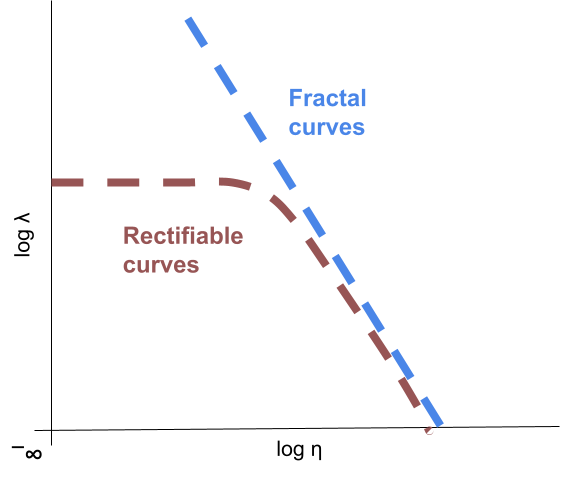
\includegraphics[width=0.6\textwidth]{Images/1.1.2.png}
  \end{center}
  \caption{The two types of curves}
\end{wrapfigure}

Curves that are nowhere rectifiable (meaning that no subset of them has a finite arc length) are called \textbf{fractal curves}, not to be confused with the general notion of a fractal which we will discuss later. Fractal curves can be contained in a finite, bounded space, yet have an infinite arc length, even when looking at a small portion of the curve. Despite expectation, as you zoom closer and closer into the image of a fractal curve, it does NOT ever begin to appear roughly linear. It will always remain \textbf{infinitely intricate}. In a calculus analogy, think of fractal curves as the graphs of functions that are everywhere continuous, but nowhere differentiable. \\

  \begin{center}
    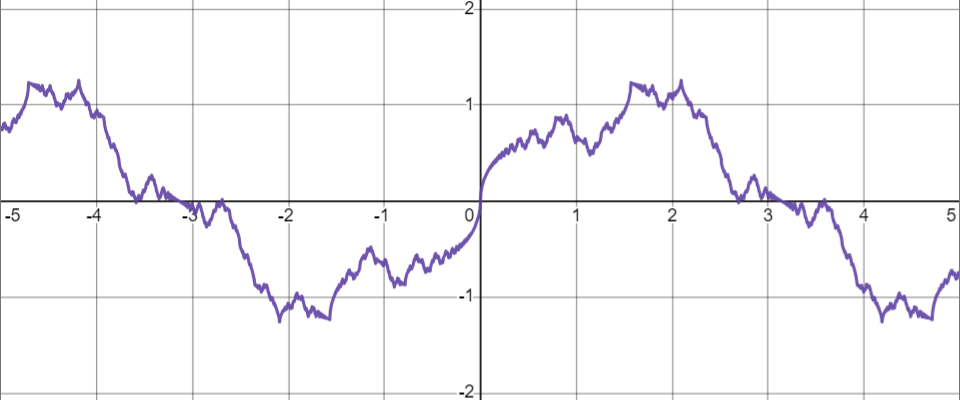
\includegraphics[width=0.75\textwidth]{Images/Chap1/1.1.2.png}
  
  \captionof{figure}{The Riemann function defined as $\sum_{n=1}^\infty \frac{\sin(n^2x)}{n^2}$ is nowhere differentiable.}
  \end{center}

Most curves fall into one of these two categories. For those that are rectifiable, as the rulers become small, the total length converges to a particular real number (notice that in Figure 1.2, the curve on the graph intersects the y-axis at a right angle). An interesting phenomenon known as Richardson's Law states that by graphing $\log\eta$ and $\log\lambda$ together, we yield something roughly linear for fractal curves. The slope of this line will have significance later when we discuss Richardson's Law.\\

\begin{exercise}
    Not all curves are in these two timcategories. Can you think of one? As a hint, try to draw a curve that has a finite number of points that are not rectifiable. 
\end{exercise}

Before we continue, we may want to define a few terms that we have been using loosely so far. When we say that a curve (or more generally, a set) is bounded, what we mean is that is that the distance between any two points in the set are at most a finite distance from each other.\\ 

\begin{definition}[Bounded Set, Diameter of a Set]
A subset $S$ of a metric space $(X,d)$ is \textbf{bounded} if there is some $r>0$ such that for any $a,b\in S$, $d(a,b)\leq r$. The \textbf{diameter} of a set is the smallest $r$ that makes this true. 
\end{definition}
\index{Bounded Set}
\index{Diameter of a Set}

Thus, the diameter of a set $(\subset \R^2)$ can be thought of as the diameter of the smallest circle enclosing the entire set. 
\begin{exercise}
    Calculate the diameter of the unit square defined by $[0,1]\times[0,1]$.
\end{exercise}
\begin{exercise}
    Given real numbers $a<b$ and $c<d$, what would the diameter of the set $[a,b]\times [c,d]$ be?
\end{exercise}
\begin{exercise} 
    We noted earlier that fractal curves, even when bounded, do not have a finite arc length. Is it necessarily the case that bounded curves that are not fractal curves must have a finite arc length? Can you find a counterexample, a curve that appears smooth, locally, but does not have a finite arc length? 
\end{exercise}

Going forward, we should be clear by what a ``curve'' is. Unfortunately though, there is no one clear definition, although depending on the context, we can create one that fits our needs best. Here, we'll be speaking in terms of general topological spaces, although we are usually just working in the usual Euclidean topology. \\

\begin{definition}[Curve]
    Suppose $(X,T)$ is a topological space. Then a curve $\Gamma$ is a continuous mapping from the set $[0,1]$ into $(X,T)$.
\end{definition}

This definition may need some explanation. The mapping we are speaking of is just some function that takes the interval $[0,1]$ and assigns a point to it. You may notice we do not specify that the function must be injective or surjective. By adding the condition of injectivity, we require that the curve does not intersect itself (or else, there is some point in $(X,T)$ that is reached at two distinct times in the curve's path). Ask yourself, why would we not specify surjectivity?\\

The function $f\ :\ [0,1]\to\E^2$ defined as $f(x)=\left(\cos(2\pi x),\sin(2\pi x)\right)$ traces out the unit circle.\\

\begin{exercise}
    Find functions $f\ :\ [0,1]\to\E^2$ that create each of the following:
    \begin{enumerate}
        \item A circle of radius $r$ and center $(h,k)$
        \item The unit square with corners at $(0,0),(0,1),(1,1),(1,0)$
        \item The line $y=1$
        \item The line with points $(a,b)$ and $(c,d)$
    \end{enumerate}
\end{exercise}

Defining infinite intricacy is a bit more challenging. In common terms, we want to describe curves that no matter how much you zoom into them, they always have a high amount of detail. Like we discussed earlier, calculus teaches students that curves usually begin to appear linear when you zoom in to small parts of them. This is how we are able to find the derivative. For fractal curves however, we will use the following definition to describe their behavior when looking at ``small'' subsets.\\ 

\begin{wrapfigure}{r}{0.4\textwidth}
  \begin{center}
    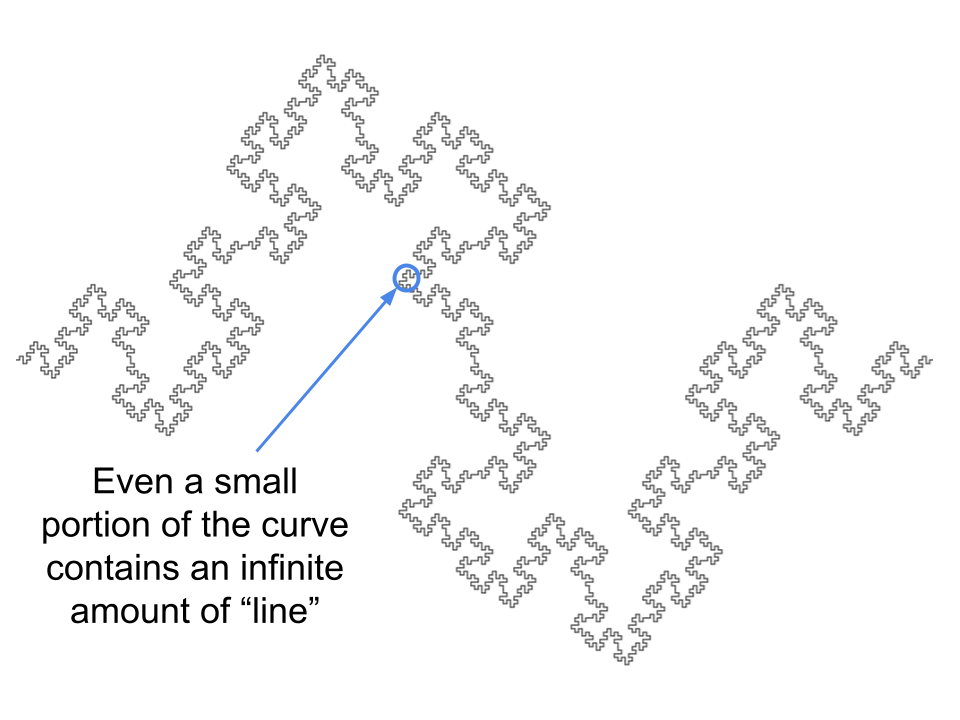
\includegraphics[width=0.4\textwidth]{Images/1.1.3.png}
  \end{center}
  \caption{The $\e$ \\neighborhood of $X\in\Gamma$}
\end{wrapfigure}

Here is a definition, using what we know about $\e$ neighborhoods\\

\begin{definition}[Infinitely-intricate]
    Suppose $\Gamma$ is a curve in $\E^n$. Then $\Gamma$ is \textbf{infinitely-intricate} if there exist uncountably many points  $X\in\Gamma$ such that for all $\e>0$, $V_\e(X)\cap \Gamma$ is not rectifiable.
\end{definition}



\begin{exercise}
    For any continuous function $g\ :\ \R\to\R$, the graph generated by plotting all points $(x,g(x))$ creates a path in $\E^2$. 
    \begin{enumerate}
        \item Prove that this path is a curve.
        \item A function is said to be \textbf{nowhere continuous} if for every $x$, there exists some $\e>0$ such that for every $\delta>0$, there is a point $c$ such that $c\in V_\delta(x)$ but $ f(c)\notin V_\e(f(x))$. Show (even if informally) that such a graph is infinitely-intricate.
    \end{enumerate}
\end{exercise}

\section{The Lebesgue Measure}
\Blindtext

\section{Topological Dimension}
\Blindtext

\clearpage

\section{Self-Similarity and Dimension}

In geometry (as opposed to the more abstract set-theory), an object is \textbf{self-similar} if a part of the object is geometrically similar to the whole. This means that you could cut out a particular portion and scale it up by a certain amount, yielding the original figure. The trivial example of a self-similar geometric object is simply that of a line segment. By cutting a line segment in half, we get two pieces that when scaled by a factor of 2, generate the original line segment. Not very interesting at all.\\

\begin{wrapfigure}{r}{0.3\textwidth}
  \begin{center}
    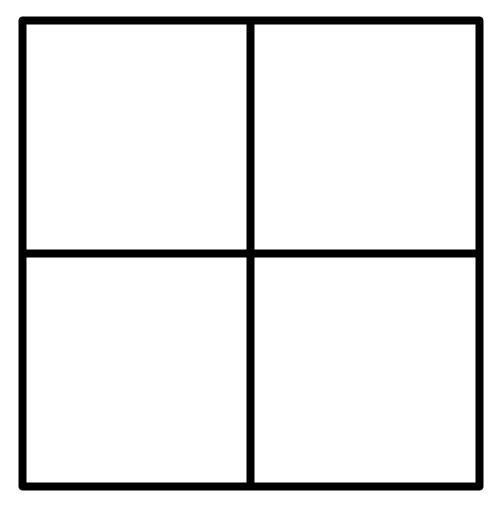
\includegraphics[width=0.3\textwidth]{Images/1.4.1.jpg}
  \end{center}
  \caption{A square is self-similar}
\end{wrapfigure}

Take a square for example, and split it into four pieces as shown to the right. Note that here, a ``square'' is referring to everything on the inside, not just the boundary. Each piece is a square (and all squares are similar to each other).  So we conclude that a square is self-similar. We could also break it into 9ths, and each square would be similar to the original by a dilation of 3.\\

You might notice that by scaling down a square by a dilation factor of $\frac{1}{n}$, you can fit exactly $n^2$ squares inside the original. The exponent of $2$ is particularly important, it represents the \textbf{fractal dimension} of the object in question. For most ordinary objects, this number is a whole number. \\

\begin{wrapfigure}{r}{0.1\textwidth}
  \begin{center}
    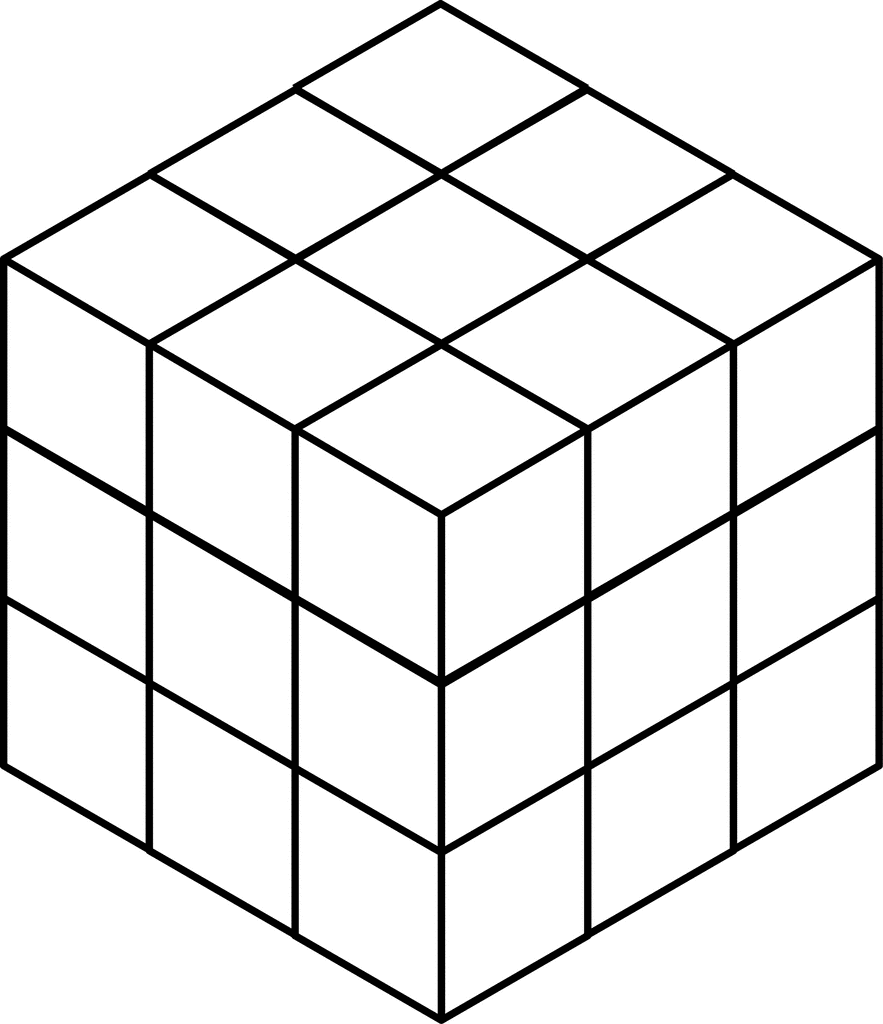
\includegraphics[width=0.1\textwidth]{Images/1.4.2.png}
  \end{center}
  \caption{27 cubes may fit into a cube 3 times as large}
\end{wrapfigure}

\begin{exercise}
    Try to do the same with an equilateral triangle. How many equal-sized equilateral triangles can you split it into? For each of these values, what is the dilation factor from each smaller piece to the whole? 
\end{exercise}



When considering a cube, we may insert $n^3$ cubes that are scaled down by a factor of $\frac{1}{n}$. The smaller cubes do not overlap, and their union creates the entire larger cube. The exponent seems to always represent the dimension of whatever object we are considering. Analogous to this, you may have noticed that geometric formulas contain these values in their exponents also. For example, the volume (Lebesgue measure 3) of a sphere of radius $r$ is $\frac{4}{3}\pi r^3$. The surface area (Lebesgue measure 2) is $4\pi r^2$. For a cylinder, the volume (Lebesgue measure 3) is $\pi r^2 h$; there are two parameters with exponents $2$ and $1$, so the dimension is $2+1=3$ (since multiplying values with exponents calls for adding the exponents together). At this point, the idea of dimension should strike a lot of connections to things taught in a standard geometry class. 

\clearpage

\begin{definition}[Self-similar]
    A set $X\subseteq \R^n$ is self-similar if there exists a proper subset $Y\subset X$ such that $X \sim Y$ (the sets are geometrically similar).
\end{definition}

\begin{example}[The unit square is self similar]
    Let $X=[0,1]\times[0,1]$, the unit square. We will consider the subset $Y=[0,0.5]\times[0,0.5]$, a proper subset of $X$. Then, by dilating every point in $Y$ about the origin by a factor of 2, we produce the set $X$. Thus, $X$ is self-similar.
\end{example}

\begin{exercise}
    Show that a line ($\R$), a rectangle ($[0,a]\times[0,b] \ a,b>0$), and a triangle (space enclosed by the lines $x=0$, $y=0$, and $x+y=1$)  are self-similar.
\end{exercise}

But in our interest of fractals, we are concerned with objects that may be self-similar, but whose dimension is non-integral, not a whole number. After all, the term fractal, coined by Benoit Mandelbrot in 1975, was named to recognize that these objects (oftentimes) have a \emph{fractional dimension}. Now consider the Cantor Set, a subset of the interval $[0,1]$ constructed recursively in the following manner. Define $C_0$ to be the interval $[0,1]$. Then for each $n\geq 1$, let $\ds C_n = \frac{C_{n-1}}{3}\cup \left(\frac{2}{3} + \frac{C_{n-1}}{3}\right)$. Then, the Cantor Set is $\ds \mathcal{C}=\lim_{n\to\infty} C_n$. \\

\begin{wrapfigure}{r}{0.4\textwidth}
  \begin{center}
    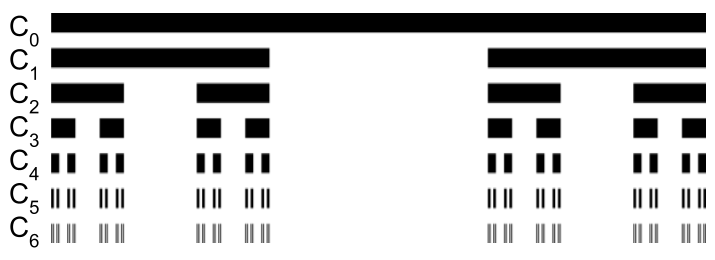
\includegraphics[width=0.4\textwidth]{Images/1.4.3.png}
  \end{center}
  \caption{Pseudo-Cantor Sets}
\end{wrapfigure}

To the right, you can see the first few iterations of $C_n$. As $n$ continues to increase, you'll notice that the set appears to be self similar. The half to the left looks like a scaled down version of the entire thing. In fact, the way $C_n$ is defined is by taking $C_{n-1}$, scaling it down by a third, making a second copy, and positioning that $2/3$ to the right. Using our intuition from earlier to find the fractal dimension of self-similar objects, the dimension of $\mathcal{C}$ is the value $D$ such that $3^D = 2$. This happens to be $\log_3(2)$ or $ \frac{\ln 2}{\ln 3} \approx 0.6309$. \\

This is mind boggling! We have just taken a look at a set whose dimension is more than $0$, but less than $1$. Our understanding of topological dimension only works for integral values, which begs the question of how one would find the topological dimension of these sets. 

\begin{exercise}
    Show that $\dim (\mathcal{C})<1$ by calculating $\lambda^*_1(\mathcal{C})$. Also calculate $\lambda^*_0(\mathcal{C})$ while you're at it.
\end{exercise}

\begin{exercise}
    Find a general formula in terms of $n$ for $\lambda^*_1(\mathcal{C}_{n})$. Does your answer to Exercise 1.4.2 match up with $\ds\lim_{n\to\infty}\lambda^*_1(\mathcal{C}_{n})$
\end{exercise}

Definition of dimension

\begin{wrapfigure}{r}{0.4\textwidth}
  \begin{center}
    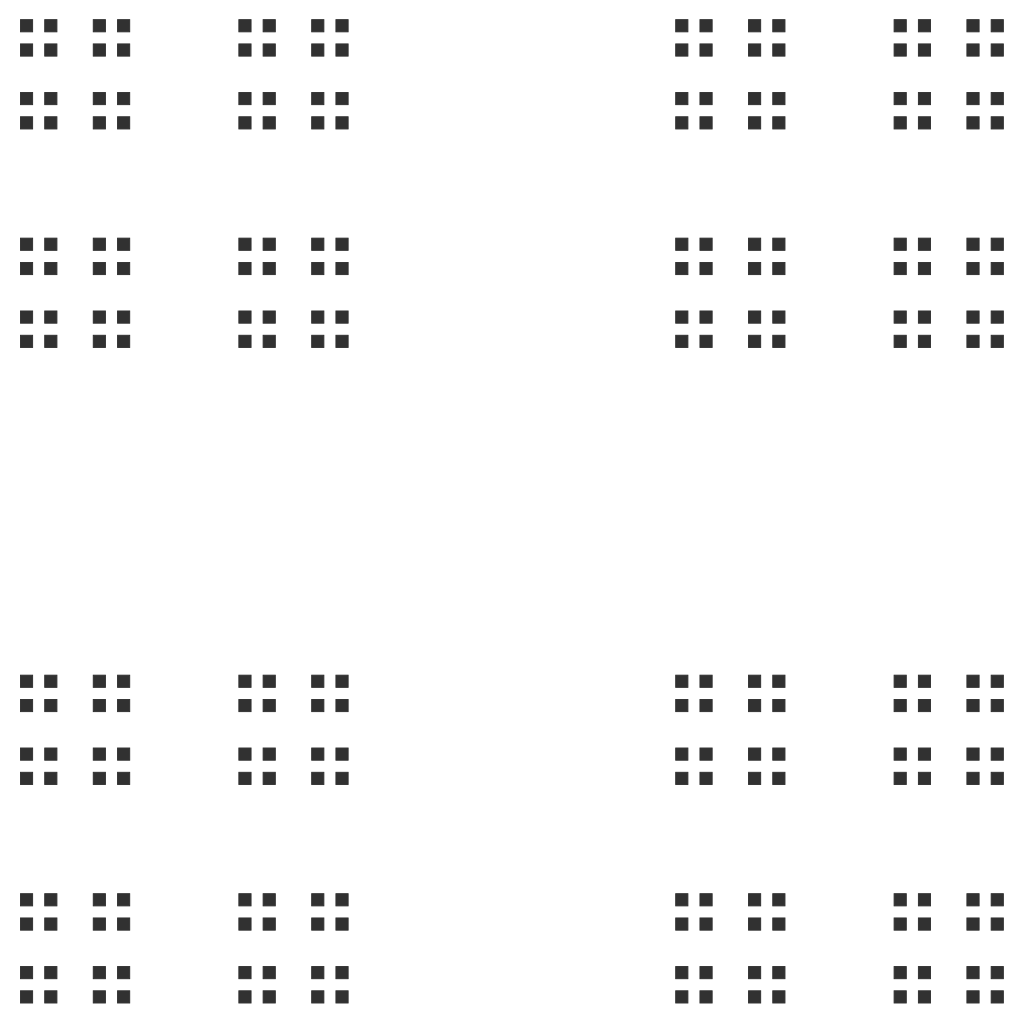
\includegraphics[width=0.4\textwidth]{Images/1.4.4.png}
  \end{center}
  \caption{The 4th iteration of Cantor Dust}
\end{wrapfigure}

To the right, we have a fractal by the name Cantor Dust. It is the next-higher-dimension set analogous to the Cantor Set. Really, what we have in the image is instead the 4th pseudo-fractal. Notice that we can generate this image by first graphing $\mathcal{C}_4$ along the $x-$axis and $\mathcal{C}_4$ along the $y-$axis. Their Cartesian product (points $(x,y)$ that such that $x\in\mathcal{C}_4$ and $y\in\mathcal{C}_4$) is shaded black. So, we can define the set to our right as $\mathcal{C}_4\times \mathcal{C}_4$ or $\mathcal{C}^2_4$. \\

Think about how each step is generated. You first start with the unit square $\mathcal{C}^2_0$, and for each iteration, you remove a ``+'', the middle third on both axes, to quadruple the number of squares. Each square is $\frac{1}{3}$ the length of the squares in the previous iteration, so each of their measures is $\frac{1}{9}$ of that in the previous step. But by quadrupling their count, the measure of each next iteration is $\frac{4}{9}$ as that of the previous. 

\begin{exercise}
    Find a general formula for $\lambda^*_2(\mathcal{C}^2_n)$. What about $\lambda^*_2(\mathcal{C}_n\times \mathcal{C}_m)$? Evaluate the limit as the iterations increase.
\end{exercise}

\begin{exercise}
    Show that $\dim(\mathcal{C}^2)<2$ by calculating $\ds \lambda^*_2(\mathcal{C}^2)$.  
\end{exercise}

\begin{exercise}
    Like we did for $\mathcal{C}$, calculate $\dim(\mathcal{C}^2)$. Compare this with $\dim(\mathcal{C})$ and come up for a general formula for $\dim(\mathcal{C}^n)$. 
\end{exercise}

\begin{wrapfigure}{r}{0.4\textwidth}
  \begin{center}
    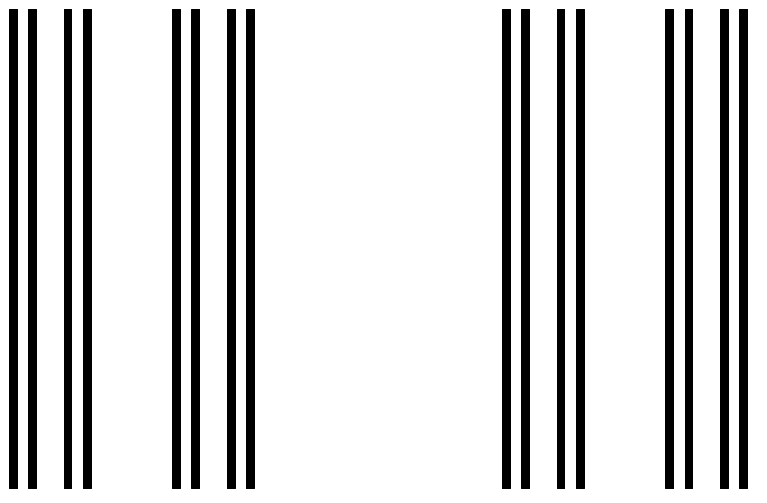
\includegraphics[width=0.4\textwidth]{Images/1.4.5.png}
  \end{center}
  \caption{$\mathcal{C}_4\times [0,0.55]$}
\end{wrapfigure}


You might have already noticed an interesting property regarding the dimensions of sets defined as the Cartesian product of two other sets. But for sake of another example, consider taking the Cantor Set and turning each point into a line segment of length 0.55. The picture to the right shows an example. We have taken the Cantor Set and simply added another dimension to it. 

\clearpage

\begin{exercise}
    Show that $\dim\left(\mathcal{C}\times [0,0.55]\right) = \dim(\mathcal{C})+\dim([0,0.55])$
\end{exercise}

Later in this text, we will prove the generalization of this theorem, particularly that for sets $A,B$, it follows that $\dim(A\times B)=\dim(A)+\dim(B)$. Although, it is not too challenging, so you can try it on your own now if you are ambitious! Otherwise, consider the exercises below to strengthen your understanding of the self-similar definition of fractals. Notice that as the name suggests, this definition only works when the set is self-similar. 

\begin{exercise}
    
\end{exercise}

\begin{exercise}
    
\end{exercise}

\begin{exercise}
    Prove that the self-similarity dimension of all rectifiable curves is 1
\end{exercise}